\documentclass{article}
\usepackage{template}

\usepackage{chngcntr} % Reset counter within sections
\usepackage{circuitikz}

\counterwithin*{equation}{section}
\counterwithin*{equation}{subsection}

\pagestyle{fancy}
\setlength\headheight{24pt}

\lhead{\className}
\rhead{\leftmark}
\cfoot{\thepage}

\newcommand{\uniTitle}{Queensland University of Technology}
\newcommand{\className}{Foundations of Electrical Engineering}
\newcommand{\classTime}{Semester 2, 2021}
\newcommand{\classInstructorName}{Dr Sam Cunningham-Nelson}
\newcommand{\authorName}{Tarang Janawalkar}
\newcommand{\authorStudentNumber}{n11032201}
\newcommand{\classCode}{EGB120}

\usepackage[
    type={CC},
    modifier={by-nc-sa},
    version={4.0},
    imagewidth={5em},
]{doclicense}

\date{}

\begin{document}
\begin{titlepage}
    \vspace*{\fill}
	\begin{center}
        \LARGE
        \textbf{\className}
        \texorpdfstring{\\}{ }
        \uniTitle
        \texorpdfstring{\\}{ }
        \texorpdfstring{\vspace{0.3in}}{ }
        \normalsize\textit{\classInstructorName}
        \texorpdfstring{\\}{ }
        \classTime
    \end{center}
    \begin{center}
        \textbf{\authorName}
    \end{center}
    \vspace*{\fill}
    \doclicenseThis
    \thispagestyle{empty}
\end{titlepage}
\newpage

\tableofcontents
\newpage

\section{Electrical Circuits}
\subsection{Fundamental Quantities}
\subsubsection{Charge}
\begin{description}
    \item[Definition.] Electric charge is a fundamental property of matter that governs how particles are affected by an electromagnetic field.
    \item[Symbol.] $q$.
    \item[Unit.] Coloumbs (\unit{\coulomb}).
    \item[Charge in an electron.] $q=\SI{1.6022e-19}{\coulomb}$. 
\end{description}
\subsubsection{Current}
\begin{description}
    \item[Definition.] Current is the rate of flow of charge.
    \item[Symbol.] $i$.
    \item[Unit.] Amps (\unit{\ampere}).
    \item[Mathematical Definition.] $i=\dv{q}{t}\iff\SI{1}{\ampere}=\SI{1}{\coulomb\per\s}$. 
\end{description}
\subsubsection{Voltage}
\begin{description}
    \item[Definition.] Voltage is the amount of energy per unit of charge. Likewise it is the potential difference in charge between two points.
    \item[Symbol.] $v$.
    \item[Unit.] Volts (\unit{\volt}).
    \item[Mathematical Definition.] $v=\dv{w}{q}\iff\SI{1}{\volt}=\SI{1}{\joule\per\coulomb}$. 
\end{description}
\subsection{Power and Energy}
\subsubsection{Power}
\begin{description}
    \item[Definition.] Power is the rate of change of energy.
    \item[Symbol.] $p$.
    \item[Unit.] Watts (\unit{\watt}).
    \item[Mathematical Definition.] $p=\dv{w}{t}\iff\SI{1}{\watt}=\SI{1}{\joule\per\s}$.
    \item[Electric Power.] $p=\dv{w}{t}=\frac{\dd{w}}{\cancel{\dd{q}}} \frac{\cancel{\dd{q}}}{\dd{t}}=vi$. 
\end{description}
\subsubsection{Passive Sign Convention}
\begin{figure}[H]
    \centering
    \begin{minipage}[H]{0.48\textwidth}
        \textbf{Passive component}
        \centering
        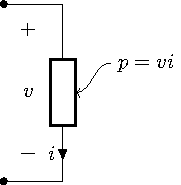
\includegraphics[height = 4cm]{passive_component}
        \caption{Energy dissipated.}
    \end{minipage}\hfill
    \begin{minipage}[H]{0.48\textwidth}
        \textbf{Active component}
        \centering
        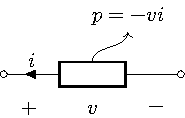
\includegraphics[height = 4cm]{active_component}
        \caption{Energy produced.}
    \end{minipage}
\end{figure}
\subsubsection{Power Balance}
\begin{theorem}
    \begin{equation*}
        p_{\text{net}} = 0
    \end{equation*}
\end{theorem}
\subsubsection{Energy}
\begin{theorem}
    \begin{equation*}
        w\left( \tau \right) = \int_0^\tau p\left( t \right) \dd{t}
    \end{equation*}
\end{theorem}
\subsection{Circuits and Sources}
\subsubsection{Circuits}
\begin{definition}
    A circuit is a mathematical model that approximates a real system. It is built from ideal circuit elements, connected by ideal wires. 
\end{definition}
\subsubsection{Voltage Source}
\begin{description}
    \item[Definition.] Produces or dissipates power at a specified voltage with whatever current is required. 
    \begin{figure}[H]
        \centering
        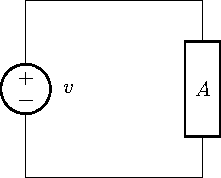
\includegraphics{voltage_source}
        \caption{Voltage Source -- $v$ is specified, $i$ varies depending on circuit element $A$.}
    \end{figure}
\end{description}
\subsubsection{Current Source}
\begin{description}
    \item[Definition.] Produces or dissipates power at a specified current with whatever voltage is required. 
    \begin{figure}[H]
        \centering
        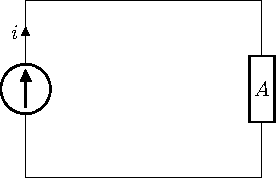
\includegraphics{current_source}
        \caption{Current Source -- $i$ is specified, $v$ varies depending on circuit element $A$.}
    \end{figure}
\end{description}
\subsubsection{Ground}
\begin{description}
    \item[Definition.] 
\end{description}
\subsubsection{Resistor}
\begin{description}
    \item[Definition.] Dissipates power so that the voltage across both terminals is proportional to the current.
\end{description}
\newpage
\section{Simple Resistive Circuits}
\newpage
\section{Diodes}
\newpage
\section{Mesh Analysis}
\newpage
\section{Source Transformation}
\newpage
\section{Inductors and Capacitors}
\newpage
\section{RC and RL Circuits}
\newpage
\section{Operational Amplifiers}
\newpage
\section{Sinusoidal Signals}
\newpage
\section{Frequency Response}
\newpage
\section{Filters and Rectifiers}
\newpage
\section{Zener Diodes and Voltage Regulators}
\newpage

\end{document}